% Options for packages loaded elsewhere
\PassOptionsToPackage{unicode}{hyperref}
\PassOptionsToPackage{hyphens}{url}
%
\documentclass[
]{article}
\usepackage{amsmath,amssymb}
\usepackage{iftex}
\ifPDFTeX
  \usepackage[T1]{fontenc}
  \usepackage[utf8]{inputenc}
  \usepackage{textcomp} % provide euro and other symbols
\else % if luatex or xetex
  \usepackage{unicode-math} % this also loads fontspec
  \defaultfontfeatures{Scale=MatchLowercase}
  \defaultfontfeatures[\rmfamily]{Ligatures=TeX,Scale=1}
\fi
\usepackage{lmodern}
\ifPDFTeX\else
  % xetex/luatex font selection
\fi
% Use upquote if available, for straight quotes in verbatim environments
\IfFileExists{upquote.sty}{\usepackage{upquote}}{}
\IfFileExists{microtype.sty}{% use microtype if available
  \usepackage[]{microtype}
  \UseMicrotypeSet[protrusion]{basicmath} % disable protrusion for tt fonts
}{}
\makeatletter
\@ifundefined{KOMAClassName}{% if non-KOMA class
  \IfFileExists{parskip.sty}{%
    \usepackage{parskip}
  }{% else
    \setlength{\parindent}{0pt}
    \setlength{\parskip}{6pt plus 2pt minus 1pt}}
}{% if KOMA class
  \KOMAoptions{parskip=half}}
\makeatother
\usepackage{xcolor}
\usepackage[margin=1in]{geometry}
\usepackage{color}
\usepackage{fancyvrb}
\newcommand{\VerbBar}{|}
\newcommand{\VERB}{\Verb[commandchars=\\\{\}]}
\DefineVerbatimEnvironment{Highlighting}{Verbatim}{commandchars=\\\{\}}
% Add ',fontsize=\small' for more characters per line
\usepackage{framed}
\definecolor{shadecolor}{RGB}{248,248,248}
\newenvironment{Shaded}{\begin{snugshade}}{\end{snugshade}}
\newcommand{\AlertTok}[1]{\textcolor[rgb]{0.94,0.16,0.16}{#1}}
\newcommand{\AnnotationTok}[1]{\textcolor[rgb]{0.56,0.35,0.01}{\textbf{\textit{#1}}}}
\newcommand{\AttributeTok}[1]{\textcolor[rgb]{0.13,0.29,0.53}{#1}}
\newcommand{\BaseNTok}[1]{\textcolor[rgb]{0.00,0.00,0.81}{#1}}
\newcommand{\BuiltInTok}[1]{#1}
\newcommand{\CharTok}[1]{\textcolor[rgb]{0.31,0.60,0.02}{#1}}
\newcommand{\CommentTok}[1]{\textcolor[rgb]{0.56,0.35,0.01}{\textit{#1}}}
\newcommand{\CommentVarTok}[1]{\textcolor[rgb]{0.56,0.35,0.01}{\textbf{\textit{#1}}}}
\newcommand{\ConstantTok}[1]{\textcolor[rgb]{0.56,0.35,0.01}{#1}}
\newcommand{\ControlFlowTok}[1]{\textcolor[rgb]{0.13,0.29,0.53}{\textbf{#1}}}
\newcommand{\DataTypeTok}[1]{\textcolor[rgb]{0.13,0.29,0.53}{#1}}
\newcommand{\DecValTok}[1]{\textcolor[rgb]{0.00,0.00,0.81}{#1}}
\newcommand{\DocumentationTok}[1]{\textcolor[rgb]{0.56,0.35,0.01}{\textbf{\textit{#1}}}}
\newcommand{\ErrorTok}[1]{\textcolor[rgb]{0.64,0.00,0.00}{\textbf{#1}}}
\newcommand{\ExtensionTok}[1]{#1}
\newcommand{\FloatTok}[1]{\textcolor[rgb]{0.00,0.00,0.81}{#1}}
\newcommand{\FunctionTok}[1]{\textcolor[rgb]{0.13,0.29,0.53}{\textbf{#1}}}
\newcommand{\ImportTok}[1]{#1}
\newcommand{\InformationTok}[1]{\textcolor[rgb]{0.56,0.35,0.01}{\textbf{\textit{#1}}}}
\newcommand{\KeywordTok}[1]{\textcolor[rgb]{0.13,0.29,0.53}{\textbf{#1}}}
\newcommand{\NormalTok}[1]{#1}
\newcommand{\OperatorTok}[1]{\textcolor[rgb]{0.81,0.36,0.00}{\textbf{#1}}}
\newcommand{\OtherTok}[1]{\textcolor[rgb]{0.56,0.35,0.01}{#1}}
\newcommand{\PreprocessorTok}[1]{\textcolor[rgb]{0.56,0.35,0.01}{\textit{#1}}}
\newcommand{\RegionMarkerTok}[1]{#1}
\newcommand{\SpecialCharTok}[1]{\textcolor[rgb]{0.81,0.36,0.00}{\textbf{#1}}}
\newcommand{\SpecialStringTok}[1]{\textcolor[rgb]{0.31,0.60,0.02}{#1}}
\newcommand{\StringTok}[1]{\textcolor[rgb]{0.31,0.60,0.02}{#1}}
\newcommand{\VariableTok}[1]{\textcolor[rgb]{0.00,0.00,0.00}{#1}}
\newcommand{\VerbatimStringTok}[1]{\textcolor[rgb]{0.31,0.60,0.02}{#1}}
\newcommand{\WarningTok}[1]{\textcolor[rgb]{0.56,0.35,0.01}{\textbf{\textit{#1}}}}
\usepackage{graphicx}
\makeatletter
\def\maxwidth{\ifdim\Gin@nat@width>\linewidth\linewidth\else\Gin@nat@width\fi}
\def\maxheight{\ifdim\Gin@nat@height>\textheight\textheight\else\Gin@nat@height\fi}
\makeatother
% Scale images if necessary, so that they will not overflow the page
% margins by default, and it is still possible to overwrite the defaults
% using explicit options in \includegraphics[width, height, ...]{}
\setkeys{Gin}{width=\maxwidth,height=\maxheight,keepaspectratio}
% Set default figure placement to htbp
\makeatletter
\def\fps@figure{htbp}
\makeatother
\setlength{\emergencystretch}{3em} % prevent overfull lines
\providecommand{\tightlist}{%
  \setlength{\itemsep}{0pt}\setlength{\parskip}{0pt}}
\setcounter{secnumdepth}{-\maxdimen} % remove section numbering
\ifLuaTeX
  \usepackage{selnolig}  % disable illegal ligatures
\fi
\usepackage{bookmark}
\IfFileExists{xurl.sty}{\usepackage{xurl}}{} % add URL line breaks if available
\urlstyle{same}
\hypersetup{
  pdftitle={Setting BirdNET species-specific threshold},
  pdfauthor={Sunny Tseng},
  hidelinks,
  pdfcreator={LaTeX via pandoc}}

\title{Setting BirdNET species-specific threshold}
\author{Sunny Tseng}
\date{2024-12-12}

\begin{document}
\maketitle

This document provides a detailed, step-by-step guide to the methodology
and R code used in our analysis for setting species-specific thresholds
for BirdNET, as described in the accompanying publication. By sharing
these instructions and code, we aim to facilitate reproducibility and
empower researchers to apply these methods to their own datasets.

\begin{Shaded}
\begin{Highlighting}[]
\CommentTok{\# set up the library}
\FunctionTok{library}\NormalTok{(tidyverse)}
\end{Highlighting}
\end{Shaded}

\subsubsection{Step 1: Analyzing audio with
BirdNET}\label{step-1-analyzing-audio-with-birdnet}

Process your audio data using BirdNET. The BirdNET Analyzer, available
on their \href{https://github.com/kahst/BirdNET-Analyzer}{Github} page,
offers several methods for analysis. Choose the one that best suits your
setup:

\begin{itemize}
\item
  \textbf{Windows GUI}: Ideal for users on a Windows operating system,
  offering a graphical user interface for ease of use.
\item
  \textbf{birdnetR Package}: A convenient option for R users, utilizing
  the reticulate package to wrap the original Python BirdNET code.
\item
  \textbf{Python}: Recommended for users comfortable with Python,
  allowing direct use of the BirdNET API or scripts.
\end{itemize}

\subsubsection{Step 2: Validation}\label{step-2-validation}

Create a validation dataset by performing stratified sampling on the
BirdNET output. In this example, we demonstrate the process using
Northern Flicker detections:

\begin{enumerate}
\def\labelenumi{\arabic{enumi}.}
\item
  \textbf{Stratify Confidence Values}: Divide the BirdNET confidence
  scores into classes ranging from 0.1 to 1, using 0.05 increments.
\item
  \textbf{Sample Audio Segments}: Randomly select 10 audio segments from
  each confidence class. This results in a total of 180 audio segments
  for validation. Notes: In this study, 180 segments were sufficient
  given our study's scale. We recommend users evaluate their specific
  data and requirements to determine the appropriate number of segments
  for robust validation.
\end{enumerate}

This stratified sampling ensures an even distribution of confidence
values in the validation dataset, providing a representative sample for
assessing threshold.

\begin{Shaded}
\begin{Highlighting}[]
\CommentTok{\# read in the output from BirdNET}
\NormalTok{birdnet\_output }\OtherTok{\textless{}{-}} \FunctionTok{read\_csv}\NormalTok{(}\StringTok{"birdnet\_full.csv"}\NormalTok{)}

\CommentTok{\# select the target species and create a validation dataset}
\NormalTok{NOFL\_validation }\OtherTok{\textless{}{-}}\NormalTok{ birdnet\_output }\SpecialCharTok{\%\textgreater{}\%}
  \FunctionTok{filter}\NormalTok{(common\_name }\SpecialCharTok{==} \StringTok{"Northern Flicker"}\NormalTok{) }\SpecialCharTok{\%\textgreater{}\%}
  \FunctionTok{mutate}\NormalTok{(}\AttributeTok{class =} \FunctionTok{cut}\NormalTok{(}\AttributeTok{x =}\NormalTok{ confidence, }\AttributeTok{breaks =} \FunctionTok{seq}\NormalTok{(}\FloatTok{0.1}\NormalTok{, }\DecValTok{1}\NormalTok{, }\FloatTok{0.05}\NormalTok{))) }\SpecialCharTok{\%\textgreater{}\%}
  \FunctionTok{slice\_sample}\NormalTok{(}\AttributeTok{n =} \DecValTok{10}\NormalTok{, }\AttributeTok{by =}\NormalTok{ class)}
\end{Highlighting}
\end{Shaded}

(Optional) To validate BirdNET's predictions, visually or aurally
confirm whether each prediction is a True Positive (TP) or a False
Positive (FP). This involves listening to the audio segments and
examining their spectrograms. To streamline the process, we developed a
BirdNET Validation ShinyApp, which integrates audio playback and
spectrogram visualization for efficient review. Refer to the
\href{https://github.com/SunnyTseng/BirdNET_validation}{Github page} for
detailed usage:

\begin{Shaded}
\begin{Highlighting}[]
\CommentTok{\# use install.packages("PACKAGE\_NAME") if you don\textquotesingle{}t have the following required packages installed yet}
\FunctionTok{library}\NormalTok{(shiny) }
\FunctionTok{library}\NormalTok{(bslib)}
\FunctionTok{library}\NormalTok{(shinyWidgets) }
\FunctionTok{library}\NormalTok{(shinyFiles)}

\FunctionTok{library}\NormalTok{(tidyverse)}
\FunctionTok{library}\NormalTok{(DT)}
\FunctionTok{library}\NormalTok{(praise)}

\FunctionTok{library}\NormalTok{(tuneR)}
\FunctionTok{library}\NormalTok{(seewave)}

\NormalTok{shiny}\SpecialCharTok{::}\FunctionTok{runGitHub}\NormalTok{(}\StringTok{"BirdNET\_validation"}\NormalTok{, }\StringTok{"SunnyTseng"}\NormalTok{)}
\end{Highlighting}
\end{Shaded}

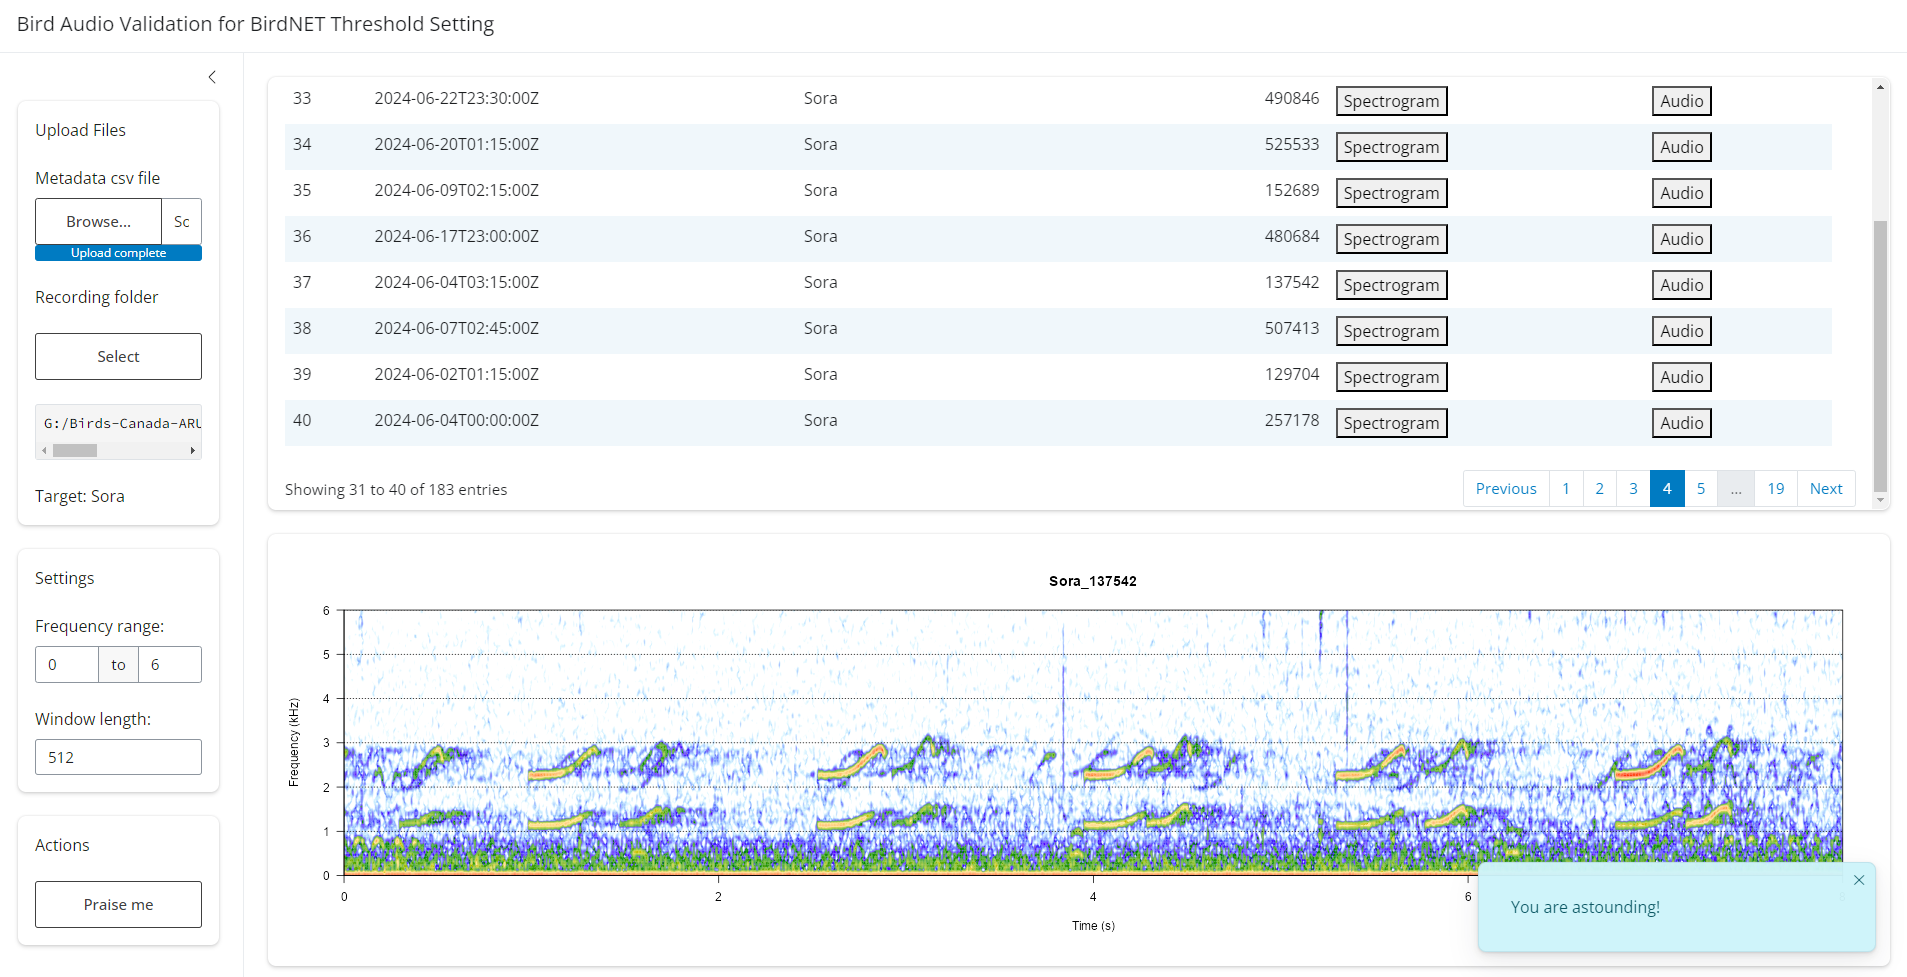
\includegraphics{images/clipboard-2461646757.png}

We used a validated Northern Flicker dataset to demonstrate the
following process. The audio data were collected from the John Prince
Research Forest in interior British Columbia, Canada.

\begin{Shaded}
\begin{Highlighting}[]
\CommentTok{\# edit the path as needed}
\NormalTok{NOFL\_validation\_finished }\OtherTok{\textless{}{-}} \FunctionTok{read\_csv}\NormalTok{(}\StringTok{"Northern\_Flicker\_finished.csv"}\NormalTok{)}
\end{Highlighting}
\end{Shaded}

\subsubsection{Step 3: Translating confidence to
probability}\label{step-3-translating-confidence-to-probability}

Apply a logistic regression model to convert BirdNET confidence scores
into probabilities, This step establishes the relationship between
BirdNET's confidence scores and the validated outcomes (True Positive or
False Positive).

\begin{Shaded}
\begin{Highlighting}[]
\CommentTok{\# fit logistic model using glm()}
\NormalTok{NOFL\_model }\OtherTok{\textless{}{-}} \FunctionTok{glm}\NormalTok{(observed }\SpecialCharTok{\textasciitilde{}}\NormalTok{ confidence, }
                  \AttributeTok{data =}\NormalTok{ NOFL\_validation\_finished, }
                  \AttributeTok{family =}\NormalTok{ binomial)}
\end{Highlighting}
\end{Shaded}

\begin{verbatim}
## `geom_smooth()` using formula = 'y ~ x'
\end{verbatim}

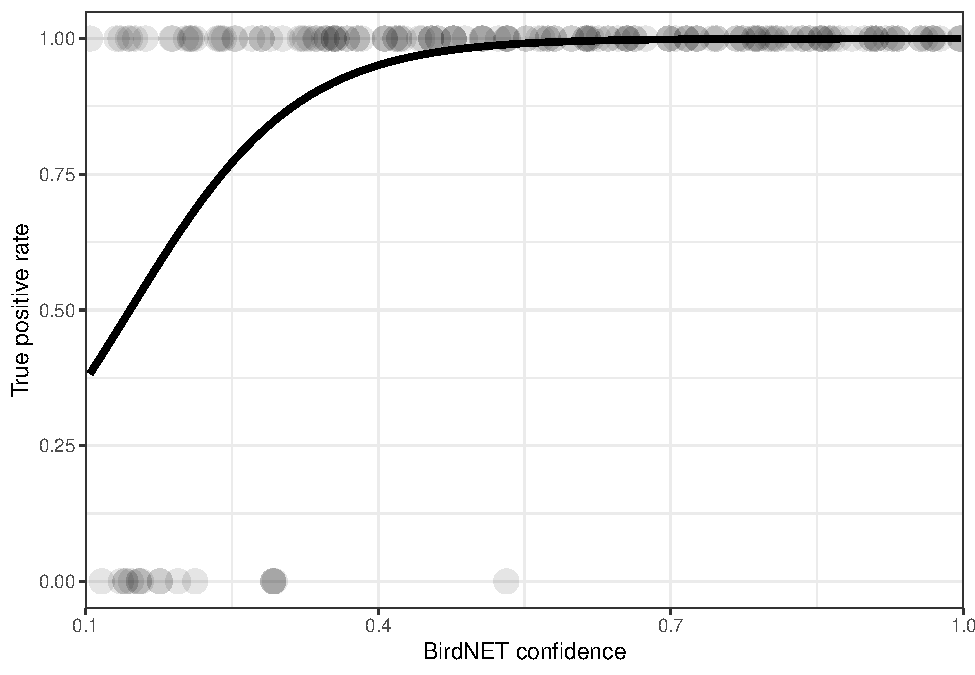
\includegraphics{species_specific_method_tutorial_files/figure-latex/unnamed-chunk-5-1.pdf}

\subsubsection{Step 4: Establishing threshold relationships with
precision}\label{step-4-establishing-threshold-relationships-with-precision}

This step calculates how different confidence thresholds influence
precision and the proportion of data retained. Using the logistic
regression model, we predict probabilities for all BirdNET outputs, then
calculate precision and the remaining data for each threshold.

\begin{Shaded}
\begin{Highlighting}[]
\CommentTok{\# find precision given a threshold}
\NormalTok{threshold2precision }\OtherTok{\textless{}{-}} \ControlFlowTok{function}\NormalTok{(probability\_data, threshold)\{}
\NormalTok{  threshold }\OtherTok{\textless{}{-}}\NormalTok{ probability\_data }\SpecialCharTok{\%\textgreater{}\%}
    \FunctionTok{filter}\NormalTok{(confidence }\SpecialCharTok{\textgreater{}}\NormalTok{ threshold) }\SpecialCharTok{\%\textgreater{}\%}
    \FunctionTok{pull}\NormalTok{(probability) }\SpecialCharTok{\%\textgreater{}\%}
    \FunctionTok{mean}\NormalTok{()}
\NormalTok{\}}


\CommentTok{\# find the data ramained given a threshold}
\NormalTok{threshold2remain }\OtherTok{\textless{}{-}} \ControlFlowTok{function}\NormalTok{(probability\_data, threshold)\{}
\NormalTok{  remain }\OtherTok{\textless{}{-}}\NormalTok{ probability\_data }\SpecialCharTok{\%\textgreater{}\%}
    \FunctionTok{filter}\NormalTok{(confidence }\SpecialCharTok{\textgreater{}}\NormalTok{ threshold) }\SpecialCharTok{\%\textgreater{}\%}
    \FunctionTok{nrow}\NormalTok{()}
  
\NormalTok{  remain}\SpecialCharTok{/}\FunctionTok{nrow}\NormalTok{(probability\_data)}
\NormalTok{\}}


\CommentTok{\# read the full BirdNET output file}
\NormalTok{birdnet\_output }\OtherTok{\textless{}{-}} \FunctionTok{read\_csv}\NormalTok{(}\StringTok{"birdnet\_full.csv"}\NormalTok{)}

\CommentTok{\# predict probabilities for Northern Flicker data}
\NormalTok{NOFL\_probability }\OtherTok{\textless{}{-}}\NormalTok{ birdnet\_output }\SpecialCharTok{\%\textgreater{}\%}
  \FunctionTok{filter}\NormalTok{(common\_name }\SpecialCharTok{==} \StringTok{"Northern Flicker"}\NormalTok{) }\SpecialCharTok{\%\textgreater{}\%}
  \FunctionTok{mutate}\NormalTok{(}\AttributeTok{probability =} \FunctionTok{predict}\NormalTok{(NOFL\_model, }\AttributeTok{newdata =}\NormalTok{ ., }\AttributeTok{type =} \StringTok{"response"}\NormalTok{)) }

\CommentTok{\# create a table of thresholds with precision and data retention}
\NormalTok{threshold\_table }\OtherTok{\textless{}{-}} \FunctionTok{tibble}\NormalTok{(}\AttributeTok{threshold =} \FunctionTok{seq}\NormalTok{(}\DecValTok{0}\NormalTok{, }\DecValTok{1}\NormalTok{, }\FloatTok{0.001}\NormalTok{)) }\SpecialCharTok{\%\textgreater{}\%}
  \FunctionTok{mutate}\NormalTok{(}\AttributeTok{data\_remained =} \FunctionTok{map\_dbl}\NormalTok{(}\AttributeTok{.x =}\NormalTok{ threshold, }
                                 \AttributeTok{.f =}\SpecialCharTok{\textasciitilde{}} \FunctionTok{threshold2remain}\NormalTok{(NOFL\_probability, .x))) }\SpecialCharTok{\%\textgreater{}\%}
  \FunctionTok{mutate}\NormalTok{(}\AttributeTok{precision =} \FunctionTok{map\_dbl}\NormalTok{(}\AttributeTok{.x =}\NormalTok{ threshold, }
                             \AttributeTok{.f =}\SpecialCharTok{\textasciitilde{}} \FunctionTok{threshold2precision}\NormalTok{(NOFL\_probability, .x)))}
\end{Highlighting}
\end{Shaded}

\begin{verbatim}
## tibble [1,001 x 3] (S3: tbl_df/tbl/data.frame)
##  $ threshold    : num [1:1001] 0 0.001 0.002 0.003 0.004 0.005 0.006 0.007 0.008 0.009 ...
##  $ data_remained: num [1:1001] 1 1 1 1 1 1 1 1 1 1 ...
##  $ precision    : num [1:1001] 0.684 0.684 0.684 0.684 0.684 ...
\end{verbatim}

\subsubsection{Step 5: Determining threshold given desired
precision}\label{step-5-determining-threshold-given-desired-precision}

To identify the confidence threshold required to achieve a specified
level of precision, we employed a generalized linear model (GLM) with a
binomial link function. This approach estimates the relationship between
confidence thresholds and precision, enabling the calculation of
thresholds for any desired precision level.

\begin{Shaded}
\begin{Highlighting}[]
\CommentTok{\# function to determine the threshold given specified precision level}
\NormalTok{precision2threshold }\OtherTok{\textless{}{-}} \ControlFlowTok{function}\NormalTok{(threshold\_table, precision)\{}
\NormalTok{  model }\OtherTok{\textless{}{-}} \FunctionTok{glm}\NormalTok{(precision }\SpecialCharTok{\textasciitilde{}}\NormalTok{ threshold, }
               \AttributeTok{data =}\NormalTok{ threshold\_table,}
               \AttributeTok{family =}\NormalTok{ binomial)}
    
\NormalTok{  (}\FunctionTok{log}\NormalTok{(precision}\SpecialCharTok{/}\NormalTok{(}\DecValTok{1} \SpecialCharTok{{-}}\NormalTok{ precision)) }\SpecialCharTok{{-}}\NormalTok{ model}\SpecialCharTok{$}\NormalTok{coefficients[}\DecValTok{1}\NormalTok{])}\SpecialCharTok{/}\NormalTok{model}\SpecialCharTok{$}\NormalTok{coefficients[}\DecValTok{2}\NormalTok{]}

\NormalTok{\}}
\end{Highlighting}
\end{Shaded}

Using this method, we determined thresholds corresponding to precision
levels of 0.9, 0.95, and 0.99. These thresholds were visualized (red for
0.9, blue for 0.95, and green for 0.99) alongside the
precision-threshold relationship.

\begin{Shaded}
\begin{Highlighting}[]
\CommentTok{\# thresholds for precision = 0.9 (red), 0.95 (blue), and 0.99 (green)}
\NormalTok{t\_0}\FloatTok{.9} \OtherTok{\textless{}{-}} \FunctionTok{precision2threshold}\NormalTok{(threshold\_table, }\FloatTok{0.9}\NormalTok{)}
\NormalTok{t\_0}\FloatTok{.95} \OtherTok{\textless{}{-}} \FunctionTok{precision2threshold}\NormalTok{(threshold\_table, }\FloatTok{0.95}\NormalTok{)}
\NormalTok{t\_0}\FloatTok{.99} \OtherTok{\textless{}{-}} \FunctionTok{precision2threshold}\NormalTok{(threshold\_table, }\FloatTok{0.99}\NormalTok{)}


\CommentTok{\# visualization of precision vs. threshold}
\FunctionTok{ggplot}\NormalTok{(threshold\_table, }\FunctionTok{aes}\NormalTok{(}\AttributeTok{x =}\NormalTok{ threshold, }
                            \AttributeTok{y =}\NormalTok{ precision)) }\SpecialCharTok{+}
  \FunctionTok{geom\_line}\NormalTok{(}\AttributeTok{stat =} \StringTok{"smooth"}\NormalTok{,}
            \AttributeTok{method =} \StringTok{"glm"}\NormalTok{, }
            \AttributeTok{se =} \ConstantTok{FALSE}\NormalTok{, }
            \AttributeTok{method.args =} \FunctionTok{list}\NormalTok{(}\AttributeTok{family =}\NormalTok{ binomial),}
            \AttributeTok{linewidth =} \FloatTok{1.5}\NormalTok{) }\SpecialCharTok{+}
  \FunctionTok{geom\_vline}\NormalTok{(}\AttributeTok{xintercept =}\NormalTok{ t\_0}\FloatTok{.9}\NormalTok{, }\AttributeTok{colour =} \StringTok{"red"}\NormalTok{, }\AttributeTok{linewidth =} \FloatTok{1.5}\NormalTok{) }\SpecialCharTok{+}
  \FunctionTok{geom\_vline}\NormalTok{(}\AttributeTok{xintercept =}\NormalTok{ t\_0}\FloatTok{.95}\NormalTok{, }\AttributeTok{colour =} \StringTok{"blue"}\NormalTok{, }\AttributeTok{linewidth =} \FloatTok{1.5}\NormalTok{) }\SpecialCharTok{+}
  \FunctionTok{geom\_vline}\NormalTok{(}\AttributeTok{xintercept =}\NormalTok{ t\_0}\FloatTok{.99}\NormalTok{, }\AttributeTok{colour =} \StringTok{"darkgreen"}\NormalTok{, }\AttributeTok{linewidth =} \FloatTok{1.5}\NormalTok{) }\SpecialCharTok{+}
  \FunctionTok{ylim}\NormalTok{(}\DecValTok{0}\NormalTok{, }\DecValTok{1}\NormalTok{) }\SpecialCharTok{+}
  \FunctionTok{theme\_bw}\NormalTok{() }\SpecialCharTok{+}
  \FunctionTok{labs}\NormalTok{(}\AttributeTok{x =} \StringTok{"Threshold"}\NormalTok{, }
       \AttributeTok{y =} \StringTok{"Precision"}\NormalTok{)}
\end{Highlighting}
\end{Shaded}

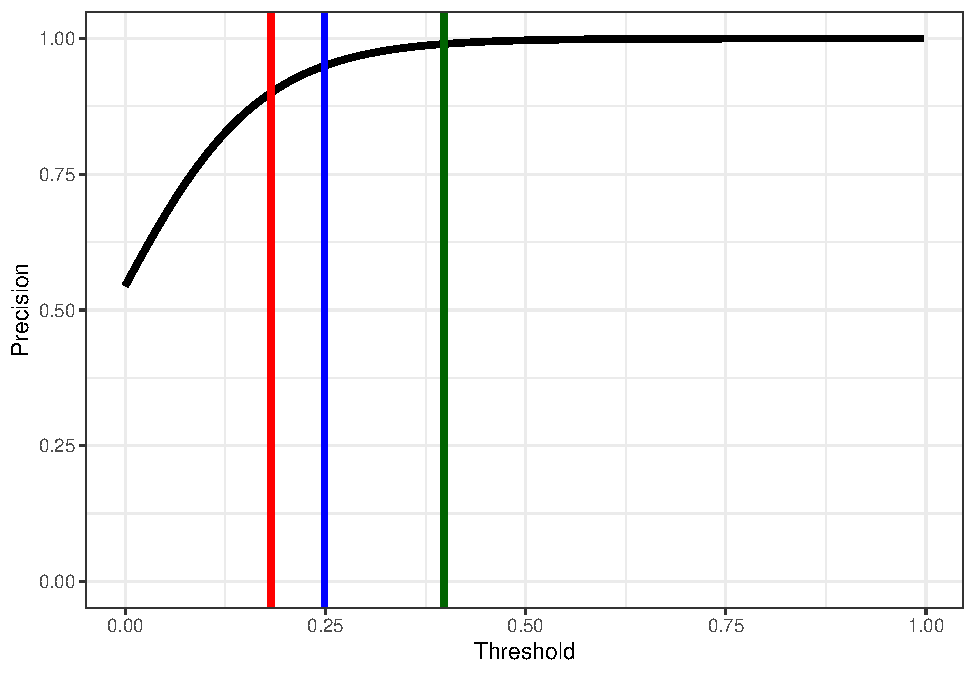
\includegraphics{species_specific_method_tutorial_files/figure-latex/unnamed-chunk-9-1.pdf}

Enjoy using BirdNET! 😃🐦😃

\end{document}
